\subsection*{Problem B6}
    \hfill \break
    To control the system a Proportional Integral Differential (PID) controller was designed. The integral part of the PID controller will adjust for physical boundaries of the system and account for systematic errors and hopefully reduce and remove offset. This helps achieve the desired characteristic set out in Problem B5. The controller was written in Python and the implementaion can be found \href{https://github.com/drlim2u/ELE2024-Control-Coursework/blob/059953dc7b2d8ba0a86b6f437153ceb4442b7a60/PartB.py#L187}{here}. The step response from the simulated controlled system was recorded and is shown below in Figure \ref{fig:problem_b6}.
    
    \begin{figure}[H]
        \centering
        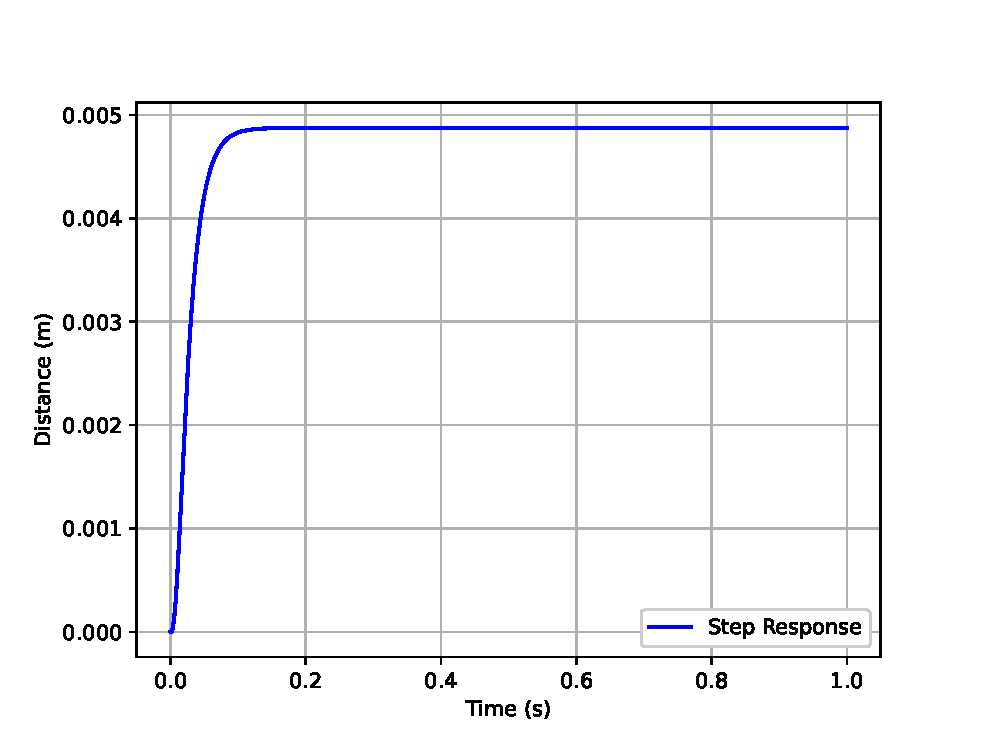
\includegraphics[width=0.6\linewidth]{figures/problem_b6.eps}
        \caption{Graph to show the step response of the system with a PID controller implemented.}
        \label{fig:problem_b6}
    \end{figure}
    
    As Figure \ref{fig:problem_b6} shows the system's impulse response settles very quickly.
